%
% main.tex -- Paper zum Thema komplexe Morlet Wavelets und CWT
%
% (c) 2019 Hochschule Rapperswil
%

\chapter{Komplexe Morlet Wavelets und CWT\label{chapter:thema}}
\lhead{Komplexe Wavelets und CWT}
\begin{refsection}
\chapterauthor{Roy Seitz}

Die schnelle Wavelettransformation (Fast Wavelet Transform, FWT) mit reellen Wavelets besitzt eine Vielzahl nützlicher Eigenschaften.
Je nach Anwendung besitzt sie jedoch auch zwei wesentliche Nachteile.

Erstens ist man sich aus der Fouriertheorie gewohnt, Phasen- und Amplitudeninformation getrennt betrachten zu können.
Diese Eigenschaft folg direkt aus der Wahl komplexer Basisfunktionen (oder Sinus und Cosinus als REal- und Imaginärteil der komplexen Schwingung) und ist mit reellen Wavelets folglich nicht möglich.

Als zweites sind die Frequenzen in der FWT nur in Zweierpotenzen der Abtastfrequenz berechnet, ähnlich der Fourier-Reihen, wo nur ganzzahlige Vielfache der Grundfrequenz berechnet werden.
Aus mathematischer Sicht ist das zwar ausreichend, für manche Anwendungen ist diese Auflösung jedoch zu grob.

Die Antworten hierzu fanden wir in Kapitel~\ref{chapter:cwt}, die kontinuierliche Wavelettransformation mit komplexen Wavelets (Continuous Wavelet Transform, CCWT).
Als erstes möchten wir folglich betrachten, wie wir mit komplexen Wavelets Amplituden- und Phasen-Information getrennt auswerten können und als zweites, wie wir geeignete Wavelets finden.

Als drittes möchten wir die CCWT effizient berechnen können.
Wir werden sehen, wie dies mittels Fourier-Transformation elegant erledigt werden kann.
Diese Berechnung liefert eine neue Interpretation der Wavelettransformation und führt zugleich zu einer Bedingung für nützliche Wavelets.

Abschliessend betrachten wir noch die Effekte der zyklischen Faltung, welche durch die FFT erzielt wird.
Dies führt zu -- möglicherweise störenden -- Randeffekten.
Deren Vermeidung ist durch padding des Sinal vermeidbar, was allerdings zusätzliche Rechenleistung erfordert.
Im letzten Teil dieses Kapitels betrachten wir folglich die Performance-Unterschiede, welche durch das PAdding entstehen.


%%%%%%%%%%%%%%%%%%%%%%%%%%%%%%%%%%%%%%%%%%%%%%%
\section{Das Morlet-Wavelet}
\rhead{Morlet Wavelet}
Auch die reellen Fourierreihen haben das Problem, dass man Amplitude und Phase nicht separat betrachten kann, wenn man nur die Cosinus-Terme verwendet.
Dies liegt daran, dass Amplitude und Phase beim Cosinus gekoppelt sind,
\[
x = A\cos(\alpha) \quad\leftrightarrow\quad \alpha = \cos^{-1}\left(\frac{x}{A}\right).
\]
Erst durch die komplexe Schwingung 
\begin{align*}
	z(t) = Ce^{i\omega t} &= |C|e^{i\left(\omega t + \arg C\right)}
%	 &= |C|\left[\cos\left(\omega t + \arg C\right) + i \sin\left(\omega t + \arg C\right)\right]
\end{align*}
erhält man eine Basisfunktion, die mit
\[
	|z(t)| = |C| \quad \text{und}\quad
	\arg z = \arg \omega t + \arg C
\]
eine separate Betrachtung von Amplitude und Winkel erlaubt.
Diese Eigneschaft überträgt sich von den Basisfunktionen auf die Fouriertransformation.
Aufgrund der eulerschen Formel
\begin{equation}
	\cos(x) = \frac{e^{ix} + e^{-ix}}{2}\label{complex:euler}
\end{equation}
kann der Cosinus aus zwei komplexen Exponentialfunktionen mit inverser Frequenz dargestellt werden.
Besitzt ein Wavelet also negative Frequenz-Anteile, dann geht bei diesen Frequenzen die Eigenschaft der Separierbarkeit von Amplitude und Phase verloren.

\begin{figure}
	\centering
	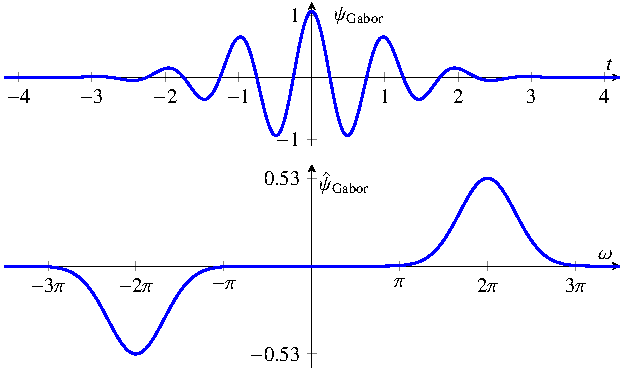
\includegraphics{papers/complex/images/gabor.pdf}
	\caption{Das Gabor-Wavelet für $\sigma = 2\pi$ \label{complex:gabor}}
\end{figure}

Ein geeignetes Wavelet benötigt folglich eine Fouriertransformierte, die bei negativen Frequenzen verschwindet.
Betrachten wir nun das Gabor-Wavelet
\[
	\psi = c_\sigma e^{-\frac{t^2}{2}}\left(\cos\left(\sigma t\right) - \kappa_\sigma\right),
\]
welches auch in Abbildung~\ref{complex:gabor} ersichtlich ist.
$c_\sigma$ und $\kappa_\sigma$ sind hierbei positive, reelle Konstanten, welche die Norm und die Zulässigkeitsbedingung~\eqref{cwt:zulaessig} korrigieren.
$\kappa_\sigma$ ist typischerweise sehr klein und wird oftmals einfach weggelassen.
Dieses Wavelet besitzt die dominante Frequenz $\sigma$ und ist durch die Gaus-Funktion in der Zeit lokalisiert.
Das Gabor-Wavelet eignet sich deshalb besonders gut, um einzelne Frequenzen in einem Signal zu finden.

Durch die Cosinus-Funktion besitzt das Gabor-Wavelet jedoch negative Frequenzen, wodurch eine isolierte Betrachtung von Amplitude und Phase unmöglich wird.
Dies möchten wir im Folgenden korrigieren.
Hierzu wechseln wir in den Fourierbereich.
Wir nutzen aus, dass die Fouriertransformierte einer Gaus-Kurve wieder eine Gauskurve ist,
\[
	\mathcal{F}\left\lbrace e^{-\alpha x^2} \right\rbrace 
	= \frac{1}{\sqrt{2\alpha}}e^{- \frac{\omega^2}{4\alpha}},
\]
und dass die Multiplikation im Zeitbereich zur Faltung im Frequenzbereich wird.
Zudem verwenden wir die Eulerformel~\eqref{complex:euler}.
Die Fouriertransformeirte des Gabor-Wavelet wird hierdurch zu
\[
 \hat{\psi} = 
 c_\sigma e^{- \frac{\omega^2}{2}} * \left(
  \frac{1}{2}\delta(\omega - \sigma) +
  \frac{1}{2}\delta(\omega + \sigma) + 
  \kappa_\sigma\delta(\omega)
  \right).
\]
Hierbei bezeichnet $\delta(\omega)$ die Dirac-Distribution.
Hieraus lässt sich der negative Anteil des Cosinus leicht entfernen.
Zudem verdoppeln wir den Anteil der positiven Frequenzen (der Grund hierfür erschliesst sich im nächsten Kapitel).
Wir erhalten
\[
	\hat{\psi}^\ast = 
	c_\sigma e^{- \frac{\omega^2}{2}} * \left(
	\delta(\omega - \sigma) +
	\kappa_\sigma\delta(\omega)
	\right),
\]
und durch Rücktransformation in den Zeitbereich
\[
	\psi^\ast = 
	c_\sigma e^{- \frac{t^2}{2}} \cdot \left(
	e^{i\sigma t} +
	\kappa_\sigma
	\right).
\]
Dies ist ein alter Bekannter, das Morlet-Wavelet aus Gleichung~\eqref{cwt:morlet}.
Abbildung~\ref{complex:morlet} zeigt den Real- und Imaginärteil, so wie die Envelope des Morlet-Wavelets.
Die Unabhängigkeit der Amplitude und der Phase 
Die Envelope entspricht hierbei gerade dem Absolutwert.
Das Morlet-Wavelet eignet sich also besonder gut, um bestimmte Frequenzen in einem Signal zu lokalisieren.
Im nächsten Kapitel werden wir sehen, dass man aus jedem, reellen Wavelet eines konstruieren kann, welches eine separate Betrachtung von Amplitude und Phase ermöglicht.

\begin{figure}
	\centering
	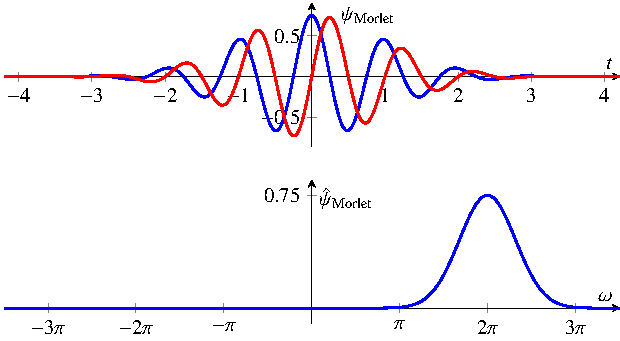
\includegraphics{papers/complex/images/morlet.pdf}
	\caption{Real- (blau) und Imaginärteil (rot) des Morlet-Wavelet für $\sigma = 2\pi$ \label{complex:morlet}}
\end{figure}

\section{Analytische Wavelets und Hilbert-Transformation}
\section{Analytische Wavelets}
Im vorherigen Abschnitt haben wir negative Frequenzen als Problem identifiziert.
Am Beispiel des Gabor-Wavelets suchten wir eine Lösung und fanden so das Morlet-Wavelet.
Dazu mussten alle negativen Frequenzen aus dem Spektrum des Wavelets entfernt werden.
Wie lässt sich dieses Verfahren veralgemeinern? 

Die Signaltheorie kennt genau dieses Verfahren in der Einseitenband-Modulation.
Wir entlehnen uns von dort den Begriff des \emph{analytischen Signals}\footnote{
	Der Begriff `analytisch' ist in diesem Kapitel immer im Sinne der Signaltheorie zu verstehen, also $\forall \omega < 0 \colon \hat f (\omega) = 0 $.
	Er ist nicht zu verwechseln mit der Eigenschaft analytischer Funktionen in der Analysis.
}
und defineiren analog dazu \emph{analytische Wavelets}.

\subsection{Analytische Signale und die Hilbert-Transformation}
\rhead{Hilbert-Transformation}
Bevor wir den Begriff des analytischen Signals einführen können, benötigen wir die Hilbert-Transformation
\[
\Hilb f(t) =
\frac{1}{\pi} \CH\int_{-\infty}^{\infty}\frac{f(x)}{t-x} \mathrm{d}x.
\]
Hierbei bezeichnet $\CH\int_{-\infty}^{\infty} \dots \mathrm{d}x$ den cauchysche Hauptwert des divergenten Integrals.
Diese Integral-Transformation wird uns erlauben, zu einem reellen Signal einen Imaginärteil zu finden, so dass gerade alle negativen Frequenzen im verscheinden.
Damit sind wir bereit für die Definition des analytischen Signals.

\begin{satz}
	\label{complex:analytic-signal}
	Sei $f(t) \in \mathbb{R}$ ein reelles Signal, dann heisst
	\begin{align*}
		f^\ast(t) 
		&= (1 + i\Hilb\,)f(t)
	\end{align*}
	das $f(t)$ zugeordnete \emph{analytische Signal}.
	Die Fourier-Transformierte eines analytischen Signals verschwindet für alle negativen Frequenzen.
	\[
		\forall \omega < 0 \colon \hat{f}^\ast(\omega) = 0
	\]
\end{satz}

\begin{proof}[Beweis]
	
	Die Hilbert-Transformation besitzt die Form eines Faltungs-Integrals.
	Im Frequenzbereich wird daraus eine Multiplikation.
	Es gilt mit der Signumsfunktion $\sgn(\omega)$ und der Identität
	\begin{align*}
		\Four \frac{1}{\pi t}  &= -i\sgn(\omega), \\
		\Hilb f(t) &= \frac{1}{\pi t} * f(t)\\
		\Four\Hilb f(t) &= -i\sgn(\omega) \hat{f}(\omega).
	\end{align*}
	Für die Fourier-Transformierte $\hat f^\ast(\omega)$ gilt folglich 
	\begin{align*}
		\hat{f}^\ast(\omega) 
		&= \hat{f}(\omega) - i^2\sgn(\omega)\hat{f}(\omega)\\
		&= (1 +\sgn(\omega))\hat{f}(\omega)\qedhere
	\end{align*}
\end{proof}

\begin{lemma}\label{complex:re-f-ast}
	Die Realteile von $f(t)$ und $f^\ast(t)$ sind identisch.
\end{lemma}

\begin{proof}
	Die Hilbert-Transformation ist eine reelle Integraltransformation
	\[\Hilb\,\colon\mathbb{R}\to\mathbb{R}.\]
	Folglich gilt nach Definition
	\[\Re f^\ast(t) = f(t) \quad \text{und}\quad \Im f^\ast(t) = \Hilb f(t)\qedhere\]
\end{proof}
Lemma~\ref{complex:re-f-ast} hält fest, dass wir uns durch die Hilbert-Transformation nicht zu weit vom Originalsignal entfernen.
\section{Analytische Wavelets}
Der Operator $\Ana\,$ hat den ersten Test also bestanden.
Nun möchten wir ihn noch etwas besser verstehen.
Was genau passiert eigentlich?
Ist es Zufall, dass das Morlet- und Gabor-Wavelet so ähnlich sind?
Dass der Realteil beim Morlet-Wavelet -- bis auf Skalierung -- genau dem Gabor-Wavelet entspricht?
Eine Anforderung an den Operator $\Ana\,$ war ja, dass er das Wavelet nur so wenig wie möglich ändern soll.
Beim Gabor-Wavelet hat das funktioniert.
Aber ist diese Eigenschaft im Allgemeinen erfüllt?
Diese Fragen möchten wir in diesem Abschnitt beantworten.

Im vorherigen Abschnitt haben wir negative Frequenzen als Problem identifiziert.
Wir definierten den Operator $\Ana\,$ so, dass er genau die negativen Frequenzen entfernt und dabei die Norm erhält.
Dazu wechselten wir in den Frequenzbereich, entfernten, was wir nicht wollten, und wechselten wieder zurück.

Wie lässt sich dieses Verfahren verallgemeinern? 
Ist dieses Hin- und Herwechseln tatsächlich notwendig?
Und was ist denn der Effekt im Zeitbereich?
Hierzu machen wir einen kurzen Ausflug in die Signaltheorie.
Die Theorie der analytischen Signale liefert uns die gesuchten Antworten.


\subsection{Analytische Signale und Hilbert-Transformation}
\rhead{Hilbert-Transformation}
In der Nachrichtentechnik ist Bandbreite ein beschränktes und dadurch wertvolles Gut.
Die Spektra reeller Signale weisen aber immer eine hermitesche Symmetrie auf.
Es reicht also, die Hälfte des Spektrums eines Signals zu übertragen, etwa nur die positiven Frequenzen.
In der Signaltheorie ist dieses Verfahren unter dem Namen Einseitenband-Modulation bekannt.
Ein Nebeneffekt hierbei ist, dass der Betrag des Signals gerade der Umhüllenden entspricht.
Eine Schwingung verliert damit ihre Nullstellen, ohne aber Information zu verlieren.
Genau das möchten wir von unseren Wavelets.

Ein Signal, bei welchem die negativen Frequenzen entfernt wurden, nennt man \emph{analytisches Signal}\footnote{
	Der Begriff `analytisch' ist in diesem Kapitel immer im Sinne der Signaltheorie zu verstehen, also $\forall \omega < 0 \colon \hat f (\omega) = 0 $.
	Er ist nicht zu verwechseln mit der Eigenschaft analytischer Funktionen in der Analysis.
}.
Wir werden analog dazu \emph{analytische Wavelets} definieren und zeigen, dass der Auslöschungsoperator eben solche erzeugt.
Dadurch übertragen sich die wesentlichen Eigenschaften analytischer Signale auf unsere neuen Wavelets.

Bevor wir den Begriff des analytischen Signals einführen können, benötigen wir aber die Hilbert-Transformation.
\begin{definition}
	Der Operator
 	\[
 	\Hilb\,\colon L^2(\mathbb R) \to L^2(\mathbb R)
 	~\quad~
 	f(t) \mapsto \Hilb f(t)
 	= \frac{1}{\pi} \CH\int_{-\infty}^{\infty}\frac{f(x)}{t-x} \mathrm{d}x
 	\]
 	heisst \emph{Hilbert-Transformation}.
 	Hierbei bezeichnet $\CH\int_{-\infty}^{\infty} \dots \mathrm{d}x$ den cauchyschen Hauptwert des divergenten Integrals.
\index{Hauptwert}%
\index{Cauchy-Hauptwert}%
\end{definition}

Die Hilberttransformation ist, wie die Wavelet- oder Fouriertransformation, eine Integraltransformation.
Ein wesentlicher Unterschied besteht jedoch darin, dass sie den Raum nicht wechselt.
Es ist eine Transformation aus der Zeit in die Zeit.

Nun sind wir bereit für die Definition eines analytischen Signals.
\begin{definition}
	\label{complex:analytic-signal}
	Sei $f \in L^2(\mathbb R)$ ein reelles Signal.
	Dann heisst
	\[f^\ast = (1 + i\Hilb\,)f \]
	das $f$ zugeordnete \emph{analytische Signal}.
\end{definition}
\index{analytisches Signal}
\index{Signal, analytisch}
\begin{satz}
	Ein analytisches Signal wird durch den Auslöschungsoperator erzeugt.
	\[1 + i\Hilb\, \equiv \sqrt 2 \Ana\, \Rightarrow f^\ast \equiv \sqrt 2 \Ana f\]
\end{satz}

\begin{proof}
	Der Auslöschungsoperator wechselt in den Frequenzbereich.
	Dort berechnet er die punktweise Multiplikation mit der Signumsfunktion und wechselt wieder zurück in den Zeitbereich.
	\[\Ana\, = \mathcal{F}^{-1}\frac{1+\sgn(\omega)}{\sqrt 2}\Four\]
	
	Dies ist folglich analog zur Faltung mit der inversen Fouriertransformierten der Signumsfunktion direkt im Zeitbereich,
	\[ \Ana f(t) = f(t) * \mathcal{F}^{-1}\frac{1 + \sgn(\omega)}{\sqrt 2}. \]
	
	Mit der Identität
	\[\Four\frac{1}{\pi t} = -i\sgn(\omega)\]
	so wie der Linearität der Fouriertransformation und der Faltung folgt schliesslich
	\begin{align*}
		\sqrt 2 \Ana f(t) 
		&= f(t) * \biggl(\delta(t) + \frac{i}{\pi t} \biggr)\\
		&= f(t) + \frac{i}{\pi} \CH\int_{-\infty}^{\infty} \frac{f(x)}{t - x} \,\mathrm{d}x\\
		&= (1 + i\Hilb\,) f(t)\qedhere
	\end{align*}
\end{proof}

Jetzt haben wir endlich alles zusammen, was wir für den Satz zur Ähnlichkeit brauchen.
Wir wollten ja zeigen, dass der Auslöschungsoperator das Signal nur gerade so stark verändert, wie notwendig.
Beim Morlet-Wavelet haben wir gesehen, dass er lediglich einen passenden Imaginärteil hinzufügt und das ganze so skaliert, dass die Norm erhalten bleibt.
Das stimmt für alle Wavelets.

\begin{satz}
	Sei $\psi \in L^2(\mathbb R)$ ein reelles Wavelet. Dann sind die Realteile von $\psi$ und $\Ana\psi$ bis auf Skalierung
	\[ \psi = \sqrt 2 \Re\Ana\psi\]
identisch.
\end{satz}

\begin{proof}
	Die Hilbert-Transformation ist eine reelle Integraltransformation
	\[\Hilb\,\colon L^2(\mathbb{R}) \to L^2(\mathbb{R}).\]
	Nach Definition gilt
	\[\Ana\psi = \frac{1 + i\Hilb\,}{\sqrt 2}\psi,\]
	woraus sich nun Real- und Imaginärteil direkt ablesen lassen:
	\[\Re \Ana\psi = \frac{1}{\sqrt 2}\psi \quad \text{und}\quad \Im \Ana\psi = \frac{\Hilb }{\sqrt 2}\psi.\qedhere\]
\end{proof}

Mittels Hilbert-Transformation kann also zu einem reellen Wavelet ein passender Imaginärteil gefunden werden, so dass Amplitude und Phase separiert werden können.
Wir definieren nun noch das eigentliche Objekt unserer Begierde.

\begin{satz}
	\label{complex:analytic-wavelet}
	Sei $\psi(t)$ ein reelles Wavelet. Dann ist
	\begin{equation}
	\psi^\ast = \Ana\psi
	\end{equation}
	das $\psi$ zugeordnete \emph{analytische Wavelet}.
\index{analytisches Wavelet}%
\index{Wavelet, analytisch}%
%	\footnote{Auch hierbei ist ``analytisch'' wieder im Sinne der Signaltheorie zu verstehen, also $\forall \omega < 0 \colon \hat\psi^\ast(\omega) = 0$.}
\end{satz}

Die analytischen Wavelets erben nun all die Eigenschaften analytischer Signale, welche durch den Auslöschungsoperator erzeugt werden.
Sie erhalten einen Imaginärteil, so dass sich Phase und Amplitude separieren lassen.
Analytische Wavelets eignen sich dadurch besonders gut, um periodische Anteile in einem Signal zu finden, da die Grösse des Skalarproduktes zwischen Wavelet und Signal unabhängig ist von der Phase.

Betrachten wir zum Abschluss noch beispielhaft das Haar-Wavelet.
Die Hilbert-Transformierte des Haar-Wavelets aus Definition~\ref{complex:def-haar} ist
\begin{align*}
	\Hilb \psi_{\text{Haar}}
	&= \frac{1}{\pi} \CH\int_{-\infty}^{\infty} \frac{\psi_{\text{Haar}}(x)}{t-x} dx\\
	&= \frac{1}{\sqrt2\pi}\left( \CH\int_{-0.5}^{0} \frac{1}{t-x}dx + \CH\int_{0}^{0.5} \frac{-1}{t-x}dx \right)\\
	&= \frac{1}{\sqrt2\pi} \left( -\left[\log \left|t-x\right| \right]_{-0.5}^{0} + \left[\log\left|t-x\right| \right]_{0}^{0.5} \right)\\
	&= \frac{1}{\sqrt2\pi} \left( -\log\left|t\right| + \log\left|t+0.5\right| + \log\left|t-0.5\right| - \log\left|t\right|\right)\\
	&= \frac{1}{\sqrt2\pi} \log\left|\frac{(t+0.5)(t-0.5)}{t^2}\right|
= \frac{1}{\sqrt2\pi} \log\left|\frac{t^2-0.5^2}{t^2}\right|.
\end{align*}

Daraus folgt das dem Haar-Wavelet zugeordnete analytische Wavelet
\[\psi^\ast_{\text{Haar}} = 
\frac{1}{\sqrt{2}}\biggl(\psi_{\text{Haar}} 
+ 
\frac{i}{\pi} \log\biggl|\frac{t^2-0.5^2)}{t^2}\biggr|\biggr).\]

Das analytische Haar-Wavelet ist in Abbildung~\ref{complex:ahaar} dargestellt.
Es hat keinen kompakten Träger mehr, ist jedoch noch immer gut lokalisiert in der Zeit.

Abbildung~\ref{complex:ahaar-ex} zeigt die Wavelet-Transformation mit dem analytischen Haar-Wavelet.
Die scharfe Lokalisierung in der Zeit und die schlecht Lokalisierung in der Frequenz sind wie beim reellen Haar-Wavelet. Ebenso wie die Verschiebung zwischen $1/a$ und $f$.
Wie erwartet ist jedoch die Helligkeit nun unabhängig von der Phase.

\begin{figure}
	\centering
	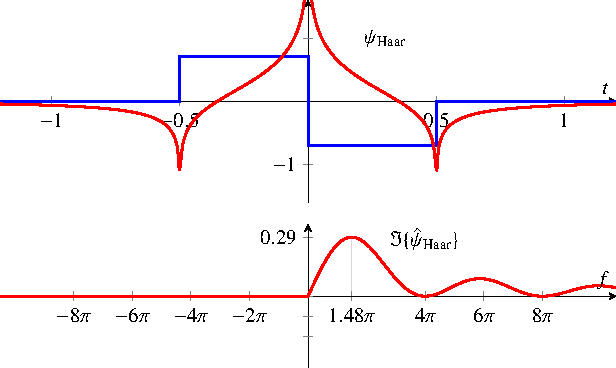
\includegraphics{papers/complex/images/ahaar.pdf}
	\caption{Das analytische Haar-Wavelet im Zeit- und Frequenzbereich.}
	\label{complex:ahaar}
\end{figure}

\begin{figure}
	\centering
	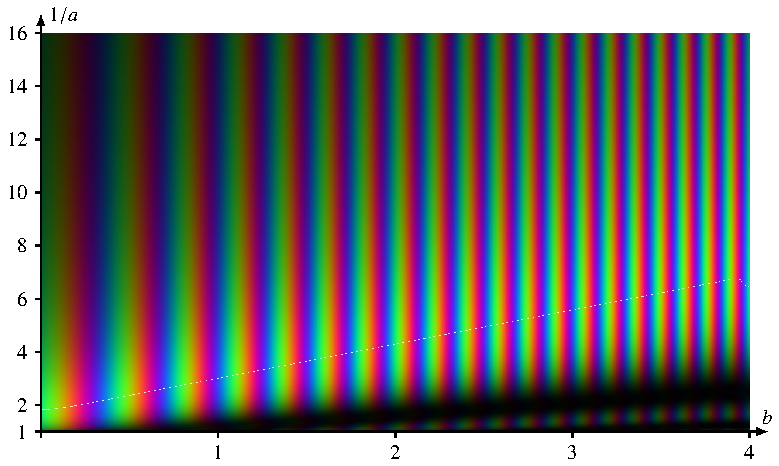
\includegraphics{papers/complex/images/chirp_ahaar.pdf}
	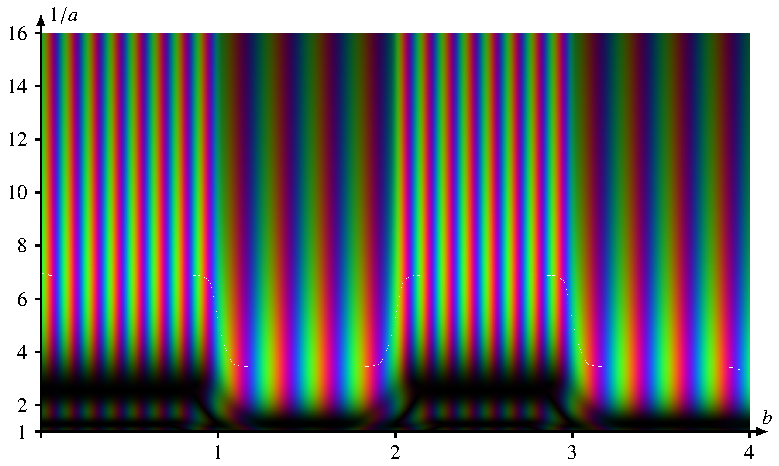
\includegraphics{papers/complex/images/square_ahaar.pdf}
	\caption{Farb-codierte Wavelet-Transformationen der beiden Beispielsignale mit dem \\ analytischen Haar-Wavelet.}
	\label{complex:ahaar-ex}
\end{figure}


\section{Schnelle Berechnung der CWT}
\rhead{Berechnung der CWT}

Betrachten wir nun die kontinuierliche Wavelet-Transformation aus Definition~\ref{cwt:definition}, Gleichung~\eqref{cwt:definition:eq},
\[
\mathcal{W}f (a,b)
=
\langle f,\psi_{a,b}\rangle
=
\frac{1}{\sqrt{|a|}}\int_{-\infty}^\infty f(t)\,
	\overline{\psi}\left(\frac{t-b}{a}\right)\,dt.
\]

Dieses Integralt entspricht der Faltung zwischen $f(t)$ und $\frac{1}{\sqrt{|a|}} \overline{\psi}\left(\frac{-t}{a}\right)$.
Die Faltung wird im Fre\-quenz\-bereich zur Multiplikation. 
Die Fouriertransformierte von $\frac{1}{\sqrt{|a|}} \overline{\psi}\left(\frac{-t}{a}\right)$ ist
\begin{align*}
	\mathcal{F}\left\lbrace \frac{1}{\sqrt{|a|}} \overline{\psi}\left(\frac{-t}{a}\right)\right\rbrace 
	&= \frac{1}{\sqrt{|a|}} \int_{-\infty}^{\infty}\overline{\psi}\left(\frac{-t}{a}\right)e^{-i\omega t}\, dt\\
	&= \frac{1}{\sqrt{|a|}} \overline{\int_{-\infty}^{\infty}\psi\left(\frac{-t}{a}\right)e^{i\omega t}\, dt}\\
	&= \frac{1}{\sqrt{|a|}} \overline{\int_{-\infty}^{\infty}\psi\left(t'\right)e^{-ia\omega t'} |a|\, dt'} \qquad \left(t' = \frac{-t}{a}\right)\\
	&= \sqrt{|a|} \, \overline{\hat{\psi}}\left(a\omega\right),
\end{align*}
 also gilt

\begin{equation}
\mathcal{W}f(a,b)
= \mathcal{F}^{-1}\left\lbrace\hat{f}(\omega)\cdot \sqrt{|a|}\, \overline{\hat{\psi}}\left(a\omega\right)\right\rbrace. \label{complex:fcwt}
\end{equation}

Mittels Fourier-Transformation lässt sich die Wavelet-Transformation also besonders elegant berechnen.
Kontinuierliche Funktionen sind für nummerische Systeme jedoch ungeeignet.
Die CWT muss also in $a$ und $b$ diskretisiert werden.
Die Diskretisierung von $b$ entspricht vorteilhaft gerade der Diskretisierung des Signals selbst.
Dann lässt sich die Fourier-Transformation mittels FFT berechnen und Gleichung~\eqref{complex:fcwt} wird zu
\begin{equation}
	\mathcal{W}f(a,b) = \text{IFFT}(\text{FFT}(f) \cdot \overline{\hat{\psi}}\left(a\omega\right))\footnote{Der Faktor $\sqrt{|a|}$ wurde hierbei weggelassen.
		Hierdurch werden die hohen Frequenzen stärker gewichtet und $|\mathcal{W}f(a,b)|$ ist gerade proportional zur Amplitude der analysierten Signalkomponente.
	}. \label{complex:ffcwt}
\end{equation}
Diese Gleichung muss für jedes $a$ einzeln gelöst werden.
Falls das Wavelet im Frequenzbereich eine geschlossene Form besitzt, wird diese Gleichung besonders interessant.
Dann benötigt man eine FFT für das Signal, und eine inverse FFT sowie eine punktweise Multiplikation mit dem Wavelet für jedes $a$.
Sei \verb|Psi_ab| eine Matrix, in deren Spalten die Fourier-Transformierten für jedes $a$ stehen, und sei \verb|f| das zu analysierende Signal $f(t)$, dann lässt sich die Wavelettransformation in Matlab oder Octave mit folgendem Code einfach berechnen
\begin{verbatim}
	function Psi_ab = myMorlet(w, a)
	  sigma = 2 * pi;
	  c_sigma = pi^(-1/4) / sqrt(1 + exp(-sigma^2) - 2 * exp(-3/4 * sigma^2));
	  w = w ./ a;
	  Psi_ab = c_sigma .* exp(-(sigma - w).^2 / 2);
	end
	
	w = linspace(0, fs, length(f))' * 2 * pi; % Column freq. vector
	a = ... ; % Interesting a values as row vector
	Psi_ab = myMorlet(w, a);
	F   = fft(f);
	yab = ifft(F .* Psi_ab);
\end{verbatim}

%% Wavelet-TraFo als Faltung zwischen Signal und Wavelet
%% Morlet-Wavelet in Frequenzbereich geschlossen berechenbar
%%  -> Faltungs-Matrix mit verschieden skalierten Morlet-Wavelets in den Spalten
%%   - Matrix-Multiplikation mit Signal
%%   - ifft über die Spalten

\section{Zyklische Faltung, Signal-Padding und Performanz}
\rhead{Zyklische Faltung}
%% Effekt der zyklischen Faltung
%% Lösen durch padden des Signals
%%  - zero padding
%%  - padden durch spiegeln des Signals
%% Performanz-Vergleich anhand Matlab-Skript

\section{Schlussfolgerung}
\rhead{Schlussfolgerung}
%% Jedes Wavelet kann in ein analytisches transformiert werden
%% Die Wavelets aus der FWT sind allerdings für die CWT ungeeignet, 
%% da sie nich in geschlossener Form im Frequenzbereich berechnet werden können
%% (Aufstellen der Faltungs-Matrix)
%% Allerdings ist das Morlet-WAvelet auch zu bevorzugen, da es die optimale 
%% Schärfe zwischen Frequenz- und Zeitauflösung beitet (Gaus\ldots)

\printbibliography[heading=subbibliography]
\end{refsection}
